\documentclass{my-cv}

\author{David Jos\'{e} da Rocha Marques}
\title{Curriculum Vitae}
\date{\today{}}

% Stop hypenation
\tolerance=1
\emergencystretch=\maxdimen
\hyphenpenalty=10000
\hbadness=10000

% Enable for xelatex
\usepackage{fontspec}
    \setmainfont{Arial}

\begin{document}
\pagenumbering{gobble}          % No page numbering
\topinfo{
  Data scientist, adept at extracting value out of raw data. Highly motivated, autodidact and quick learner. Mainly interested in applying statistical methods to solve business problems and optimize decision making under uncertainty.
}                  

\vspace{4mm}


\begin{tabular}{l|l}
\begin{minipage}[t][][b]{.35\linewidth}
    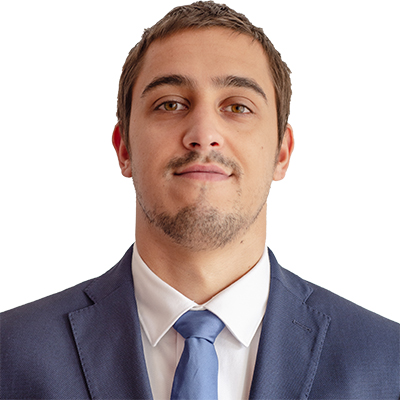
\includegraphics[width=\textwidth]{figures/david_2_linkdin.jpg} % Picture

    \vspace{2mm}

    \begin{skills}{Info}

    \nationality{Portuguese}

    \phone{+351 962 154 064}

    \email{davidmarques856@gmail.com}

    \faLinkedinSquare: \href{https://www.linkedin.com/in/djrmarques/}{/in/djrmarques}

    \faGithub: \href{https://github.com/djrmarques}{djrmarques}


    \vspace{3mm}
    \end{skills}
    % Here is the info

    \begin{skills}{Languages}

    \skillentry{Portuguese}{5}\\                                                                                                                                                   
    \skillentry{English}{5}\\
    \skillentry{German}{2}
    \end{skills}

    \begin{skills}{Programming}
    \skillentry{Python}{4}
    \skillentry{\LaTeX2}{3}
    \skillentry{Matlab}{3}
    \skillentry{HTML/CSS/JS}{2}
    \skillentry{Elisp}{2}
    \skillentry{R}{2}
    \skillentry{Scala}{2}
    \skillentry{Bash}{1}
    \skillentry{C}{1}
    \end{skills}

    \begin{skills}{Deep Learning}
    \skillentry{Keras}{3}
    \skillentry{Pytorch}{3}
    \end{skills}

    \begin{skills}{Big Data}
    \skillentry{Spark}{3}
    \skillentry{Databricks}{2}
    \end{skills}

    \begin{skills}{Database}
    \skillentry{MySQL}{3}
    \skillentry{SQL Server}{3}
    \end{skills}

    \begin{skills}{VCS}
    \skillentry{Git}{3}
    \end{skills}

    \begin{skills}{Containers}
    \skillentry{Docker}{3}\\
    \end{skills}


\end{minipage}&
\begin{minipage}[t][][t]{.65\linewidth}

  \begin{cvpart}{Experience}
  \experience{Data Scientist}{Jun/2020-Present}{\href{https://innovation.adene.pt/}{ADENE}}\\
  Solving challenges in the energy sector using data science.
  \devskills{Python, Data Visualization, Data Cleaning, Machine Learning, Git}

  \experience{Data Scientist}{Apr/2019-May/2020}{\href{https://www.closer.pt/}{Closer Consulting}}\\
  Developing solutions for various business challenges. Projects related to time series forecasting, optimization, NLP and regression analysis.
  \devskills{Python, Data Visualization, Data Cleaning, Metaheuristics, Machine Learning, \emph{SQL}, Git, Spark, Databricks, Keras}
  \end{cvpart}

  \begin{cvpart}{Projects}
    \experience{Production Plan Optimization}{}{Closer Consulting}\\
    Using metaheuristics to optimize the daily production plan of 7 factory machines.

    \experience{Transport Price Forecasting}{}{Closer Consulting}\\
    Monthly prediction of the transportation price by boat on the Rhine river.

    \experience{Datalogger Failure Analysis}{}{Closer Consulting}\\
    Using Spark to process the logs of millions of devices spread across Portugal.
  \end{cvpart}


  % Education Bit
  \begin{cvpart}{Education}
    \experience{Mechanical Engineering Masters}{2011-2018}{Energy Specialization. \\ Instituto Superior T\'{e}cnico, Lisboa, Portugal. \\ Conclusion Grade: 15/20}

    Masters with courses on optimization, machine learning, databases and operations research.
    
    \experience{Master's Dissertation}{2018}{Grade: 18/20
    }

   	Intelligent ventilation system controller based on \emph{Reinforcement Learning.}
	\devskills{Python, \emph{SQL}, Linux, \LaTeX2, Git}
  \end{cvpart}

\end{minipage}
\end{tabular}
\end{document}

%%% Local Variables: 
%%% coding: utf-8
%%% mode: latex
%%% TeX-engine: luatex
%%% TeX-master: t
%%% End: 

